\documentclass[twoside,12pt]{article}
%\documentclass{book}

\setcounter{secnumdepth}{5}

\usepackage[nottoc]{tocbibind}
\usepackage[toc,page]{appendix}
\usepackage{amsmath,amsfonts,amsthm,fullpage}
\usepackage{amsmath}
\usepackage{amssymb}
\usepackage{listings}
\setlength{\parindent}{0pt}
\usepackage{graphicx}
\usepackage{bm}
\usepackage[section]{placeins}
\usepackage{lipsum} % just for the example
\usepackage{array}
\usepackage[export]{adjustbox}
\usepackage{subfigure}
\usepackage{titlesec}
\usepackage{multirow}
\usepackage[section]{placeins}
\usepackage{tabularx} 
\usepackage{mathtools}
\usepackage[nodisplayskipstretch]{setspace}
\usepackage{color}
% Use the standard article template.
%
% The geometry package allows for easy page formatting.
\usepackage{geometry}
% Load up special logo commands.
\usepackage{doc}
% Package for formatting URLs.
\usepackage{url}
% Packages and definitions for graphics files.
\usepackage{epstopdf}



%
\geometry{letterpaper}
\setstretch{1}

\DeclareGraphicsRule{.tif}{png}{.png}{`convert #1 `dirname #1`/`basename #1 .tif`.png}

\def\argmin{\operatornamewithlimits{arg\, min}}
\newcommand{\rbr}[1]{\left(#1\right)}
\newcommand{\cbr}[1]{\left\{#1\right\}}
\newcommand{\Ncal}{\mathcal{N}}
\renewcommand{\familydefault}{\sfdefault}
\newcolumntype{L}{>{\centering\arraybackslash}m{3cm}}
\def\argmin{\operatornamewithlimits{arg\, min}}
%\newcommand\Myperm[2][n]{\prescript{#1\mkern-2.5mu}{}P_{#2}}
%\newcommand\Mycomb[2][n]{\prescript{#1\mkern-0.5mu}{}C_{#2}}
\newcommand\inv[1]{#1\raisebox{1.15ex}{$\scriptscriptstyle-\!1$}}
\newcommand\numberthis{\addtocounter{equation}{1}\tag{\theequation}}
\newcommand{\norm}[1]{\left\lVert #1 \right\rVert}

\definecolor{dkgreen}{rgb}{0,0.6,0}
\definecolor{gray}{rgb}{0.5,0.5,0.5}
\definecolor{mauve}{rgb}{0.58,0,0.82}

\lstset{frame=tb,
  language=Java,
  aboveskip=3mm,
  belowskip=3mm,
  showstringspaces=false,
  columns=flexible,
  basicstyle={\small\ttfamily},
  numbers=none,
  numberstyle=\tiny\color{gray},
  keywordstyle=\color{blue},
  commentstyle=\color{dkgreen},
  stringstyle=\color{mauve},
  breaklines=true,
  breakatwhitespace=true,
  tabsize=3
}


\setcounter{secnumdepth}{4}
\titleformat{\paragraph}
{\normalfont\normalsize\bfseries}{\theparagraph}{1em}{}
\titlespacing*{\paragraph}
{0pt}{3.25ex plus 1ex minus .2ex}{1.5ex plus .2ex}


\titlespacing\section{0pt}{2pt plus 1pt minus 1pt}{0pt plus 1pt minus 1pt}
\titlespacing\subsection{0pt}{2pt plus 1pt minus 1pt}{0pt plus 1pt minus 1pt}
\titlespacing\subsubsection{0pt}{2pt plus 1pt minus 1pt}{0pt plus 1pt minus 1pt}




%
% Set the title, author, and date.
%
\title{Analysis of a Linear Regression Model for Time Series Data}
\author{Ajay D'Souza (adsouza31)}
\author{
  D'Souza, Ajay\\
  \texttt{ajaydsouza@gatech.edu}
}
\date{}
  
\iffalse
*------------------------------------------------------------*
  These are the instructions for the Final Report
*------------------------------------------------------------*

\fi

\begin{document}

\maketitle
\begin{center}
Analysis of the suitability of a linear regression model to predict the log stock returns of one stock(GM) from the log stock returns of other stocks in the same Industry(Toyota,Ford)
\end{center}

% Add an abstract.
\begin{abstract}
From the sample time series data set of daily log returns for GM, Toyota and Ford develop a Linear Regression Model to predict the returns for GM from the returns of Toyota and Ford.  The log returns of GM is the response variable which the model should predict using the predictor variables, the log returns of Ford and Toyota.
\end{abstract}
% Add various lists on new pages.
\pagebreak
\tableofcontents

\pagebreak
\listoffigures
\listoftables

% Start the paper on a new page.
\pagebreak



%
% Body text.
%
$\\\\$
\section{Summary}
\label{summary}
 We analyze the provided daily log returns sample data to understand factors like the relationship between the variables, the distributions of the variables. We fit a simple linear model with the first degree terms of two the predictor variables Ford and Toyota. The performance and assumptions of this model are analyzed. Based on this diagnosis we fit a second linear model with a additional second degree orthonormal Polynomial term on the log returns of Toyota. We analyze the performance of the two models. We compare the performance of the two models with 10-Fold cross validation. We use this analysis and validation set results to choose the better linear model.

$\\\\$
\section{Introduction}
\label{intro}
 We are provided with a sample size of $N=709$ data points. The Preliminary data analysis shows a strong correlation between the Ford and GM log returns. The correlation between Toyota and GM and Toyota and Ford while being positive is weak. The simple linear model fitted to this data has a $\mathbf{R}^2\approxeq0.37$. ANOVA results show that almost all of the contribution to explaining the variation from the regression sum of squares in this model comes from the Ford predictor variable. For the predictor variable Toyota, both the F-value from ANOVA and the P-Value from the summary of the linear model are at around $11\%$. So the support for rejecting the NULL hypothesis and accepting that log returns of Toyota as a predictor are significant to this linear model is not very strong. 
 $\\$
 We check if the linear regression model can be enhanced by a linear relationship with a higher order polynomial term in Toyota. We generate orthonormal polynomial terms up to degree 2 for Toyota and try to fit a linear regression model to this data. We check if he linear model fitted has a better $\mathbf{R}^2$. We also check the F-Value from ANOVA and the P-Value from the summary of the linear regression to see if it offers better support for rejecting the NULL hypothesis and accepting the 2nd degree polynomial terms for Toyota as significant to this model.
 $\\$
 For both models we check for deviation from our model assumptions of normality, constant variance, linearity by a using plots of the studentized residuals against fitted values, predictors, density and QQ plots with normal distribution. We check for high leverage points, residual outliers and data points with high influence using the plots for hat matrix values, Studentized Residuals and Cooks Distance.
 $\\$
 Finally we do robust comparison of the 2 models using a 10 Fold cross validation. The Mean Residual Square Error (MSE) on the all the hold out validation test sets in each fold is used as the metric for evaluating model performance.
$\\$
\section{Body}
\label{body}
\subsection{Data Analysis}
\label{data_analysis}
The sample dataset has $N=709$ data points. The following is the correlation matrix for the log returns of Ford,Toyota and GM. There is a strong linear correlation of $0.61$ between Ford and GM. There is a weak linear correlation of $0.20$ between Toyota and GM and weak correlation of $0.24$ between Toyota and Ford.
\begin{verbatim}
Correlation:
> cor(cbind(Toyota,Ford,GM))
       Toyota Ford   GM
Toyota   1.00 0.24 0.20
Ford     0.24 1.00 0.61
GM       0.20 0.61 1.00
\end{verbatim}


\pagebreak
\FloatBarrier
{
The following figure $\eqref{fig:hw5_pairs}$ is the density and scatter plot of the daily log returns sample data. The scatter plot shows the positive correlation between Ford and GM and weak correlation between Toyota and GM and Toyota and Ford. The Density plots for each of the three variables shows a density distribution with thick tails. The GM and Ford data shows a slight skew.The Toyota distribution appears to be fairly symmetric
\begin{figure}[htbp!]
     \begin{center}
            \hspace*{-1.5in}
            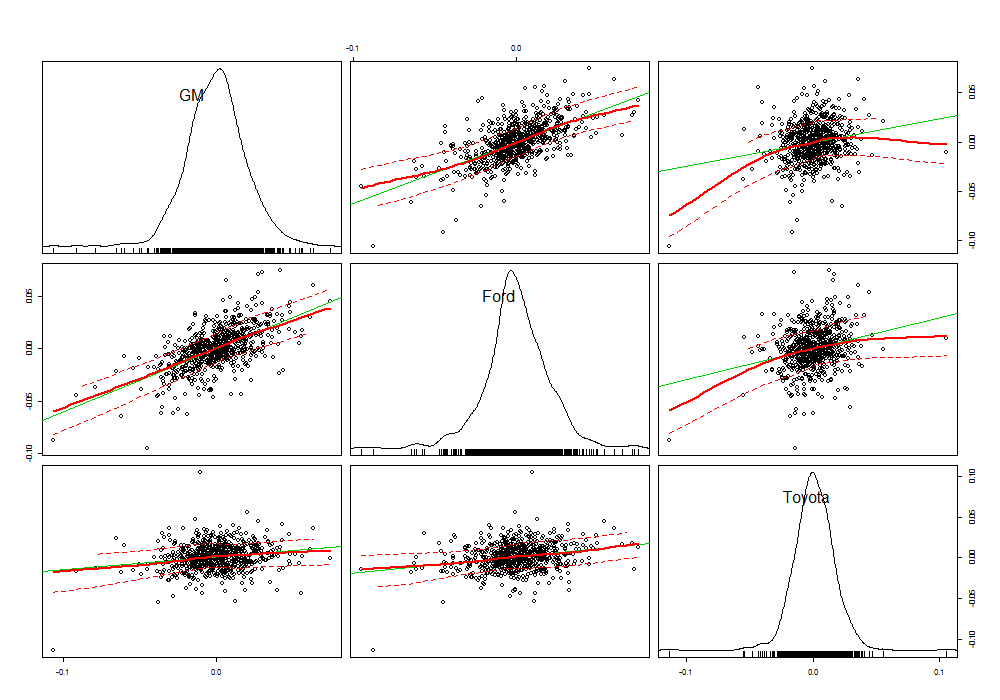
\includegraphics[width=1.35\textwidth]{charts/hw5_g_pairs}
    \end{center}
    \caption{%
     Correlation and Density Plots of of Toyota, Ford and GM log Returns
     }%
   \label{fig:hw5_pairs}
\end{figure}
}

\FloatBarrier
{
Figure $\eqref{fig:hw5_qq}$ is the QQ plot for the sample data with both a Normal and  T distribution with $\nu=4$. All plots appear thick tailed. GM and Ford data seem to be closer in their distribution.  The body and shoulders for Toyota plot is straighter and a better fit for both the normal and T distribution compared to GM and Ford data.
\begin{figure}[htbp!]
     \begin{center}
           \hspace*{-1.0in}
           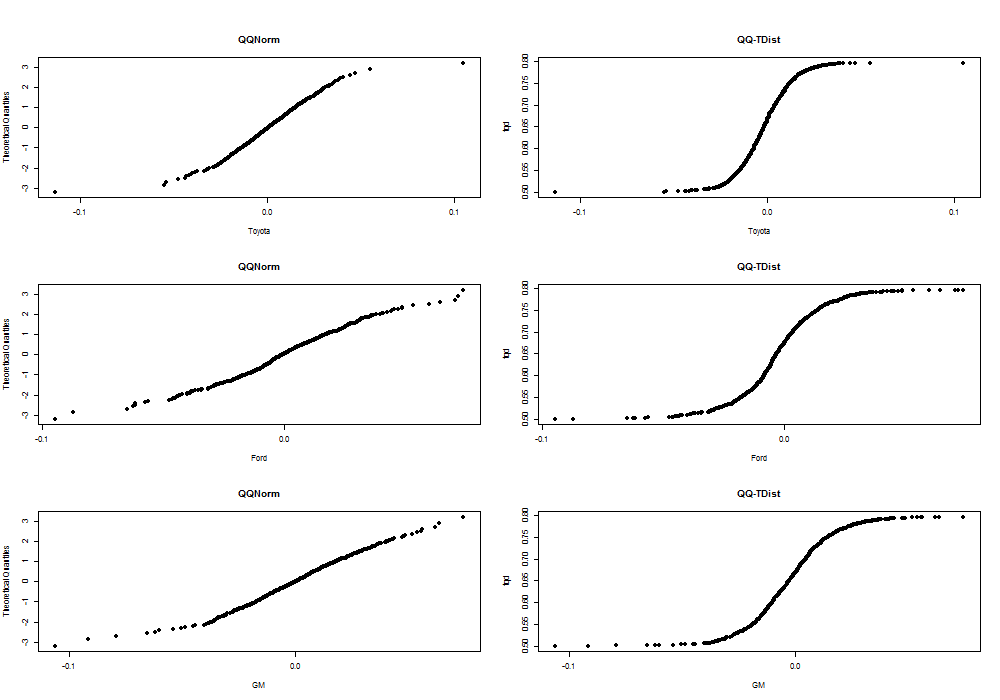
\includegraphics[width=1.4\textwidth]{charts/hw5_g_qq}
    \end{center}
    \caption{%
     QQ Plots - of Toyota, Ford and GM log Returns Vs Normal and T Distribution with $\nu=4$
     }%
   \label{fig:hw5_qq}
\end{figure}
}

\FloatBarrier
$\\\\$
\subsection{Analysis of the simple Linear Regression Model}
\label{analysis_lm_model}

\FloatBarrier
$\\$
\subsubsection{Model Selection - Predictor Subset}
\label{model_predictor_subset_1}
Since we have just 2 predictor variables, model selection for the simple linear regression model simply involves  choosing either the best 1 predictor variable model or the 2 predictor model. The $leaps()$ call in R, chooses the best k-subset of predictor variables for each $k\in1\dots2$. The following are the results of $leaps()$ function. The best k-Subset predictors are listed along with their $\mathbb{C}_p$ values.
\begin{verbatim}
Leaps - Best Model for each K Predictor by Cp:
  Ford Toyota    
1    1      0 3.6
2    1      1 3.0
\end{verbatim}
$\\$
Similar selection of the best k-subset of predictors can be performed using the $regsubsets()$ call in R.Results are attached below. In both cases as expected we see that for a 1 predictor model, Ford is the better linear predictor for GM log returns than Toyota.
\begin{verbatim}
Regression Subsets - Choosing the Best set of Predictors:
Subset selection object
Call: regsubsets.formula(data$GM ~ ., data = as.data.frame(cbind(data$Ford, 
    data$Toyota)), nbest = 1)
2 Variables  (and intercept)
   Forced in Forced out
V1     FALSE      FALSE
V2     FALSE      FALSE
1 subsets of each size up to 2
Selection Algorithm: exhaustive
         V1  V2 
1  ( 1 ) "*" " "
2  ( 1 ) "*" "*"
\end{verbatim}
$\\$
\FloatBarrier
{
We choose the best subset of predictors, among these two 1-Predictor and 2-Predictor models by comparing the $\mathbf{R}^2$ results and along with AIC, BIC and $\mathbb{C}_p$ model quality measures. For  $\mathbf{R}^2$, a higher value is better, for the AIC, BIC and $\mathbb{C}_p$, a lower value indicates a better model.Figure $\eqref{fig:hw5_m1_g_model_selection}$ plots these values.
\begin{figure}[htbp!]
     \begin{center}
             \hspace*{-0.9in}
            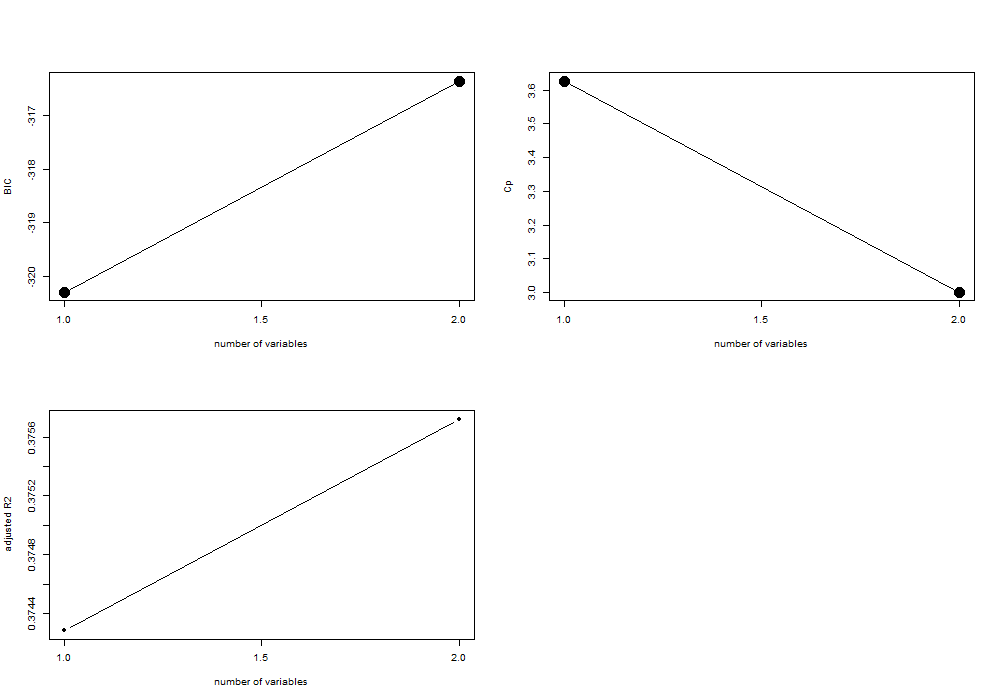
\includegraphics[width=1.35\textwidth]{charts/hw5_m1_g_complexity}
    \end{center}
    \caption{%
    Plot of No of Predictor Variables Vs BIC, $\mathbf{C}_p$ , $\mathbf{R}^2$ 
     }%
   \label{fig:hw5_m1_g_model_selection}
\end{figure}
}

\subsubsection{Model Selection - AIC}
\label{stepaic_1}
The most parsimonious model is the model with the lowest AIC value. The $stepAIC()$ R call systematically removes one predictor variable at a time till the AIC stops reducing. The following results of the $stepAIC()$ call show that the 2 predictor variable model has the lowest AIC of -5885.44.
\begin{verbatim}
Step AIC  GM ~ Ford + Toyota :
Start:  AIC=-5885.44
GM ~ Ford + Toyota

         Df Sum of Sq    RSS   AIC
<none>                0.1745 -5885
- Toyota  1   0.00065 0.1752 -5885
- Ford    1   0.09515 0.2697 -5579

\end{verbatim}

$\\$
All of the model selection criteria considered above suggest that the model having both the predictors Ford and Toyota is a slightly better choice than the 1 predictor model with only Ford as the predictor.

$\\$
\FloatBarrier
\subsubsection{Model Selection -ANOVA}
We can use ANOVA to compare the model with only Ford as the predictor with the 2-predictor model
having both Ford and Toyota. The ANOVA results show that the $\mathbf{R}^2\approxeq0.37$. So close to $37\%$ of the total variance in GM can be explained by the predictor model having both Ford and Toyota as predictors.
The increase regression sum of squares with the 2-predictor model is 0.0006492. This is very small compared to the regression sum of squares of 0.10518 from the model with only Ford. The F-Value for the Null hypothesis is $0.106 \approxeq 11\%$. So we can accept the 2-predictor model as significant and reject the Null hypothesis at the $11\%$ level, which is weak. A smaller F-value would have suggested a stronger support for the 2-predictor model.
\begin{verbatim}
ANOVA for the linear regression model : GM ~ Ford + Toyota :
Analysis of Variance Table

Response: GM
           Df  Sum Sq Mean Sq F value Pr(>F)    
Ford        1 0.10518 0.10518 425.482 <2e-16 ***
Toyota      1 0.00065 0.00065   2.626  0.106    
Residuals 706 0.17453 0.00025                   
---
Signif. codes:  0 ‘***’ 0.001 ‘**’ 0.01 ‘*’ 0.05 ‘.’ 0.1 ‘ ’ 1
\end{verbatim}

\FloatBarrier
\subsubsection{VIF}
The Variance Inflation Factor (VIF) for both Ford and Toyota are very close to 1. This confirms what
we have seen earlier with the correlation that the predictor variables Ford and Toyota are not very
well correlated to one another and one cannot be predicted from the other. This means that the
standard deviation of the estimated slope of one is not much affected by the presence of the other
in the model. So the quality of prediction of the response is not much affected by
having both the predictor variables in the model.
\begin{verbatim}
Variance Inflation Factor:
   Ford  Toyota 
1.06246 1.06246 
\end{verbatim}

\FloatBarrier
\subsubsection{Partial Residual Plot}
{
 Figure $\eqref{fig:hw5_m1_g_partial_residual}$ plots the partial residuals for his model. The plot in (b) has a slightly shallower slope than in plot (d). This shows that when predictor variable Ford is in the model, the effect of Toyota on the response variable GM is less than when Ford is not in the model. This is due to the slight collinearity that exists between the Ford and Toyota Predictor Variables. The same effect but to a much smaller degree can be seen in plots (a) and plot(c) for Ford and GM.
\begin{figure}[htbp!]
     \begin{center}
     \hspace*{-1.3in}
            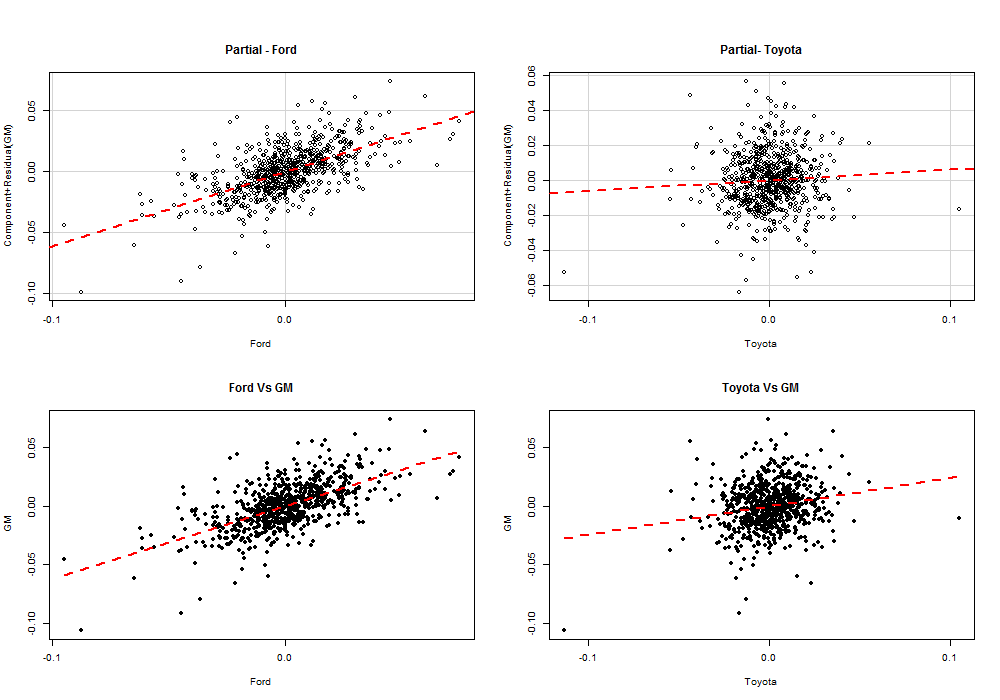
\includegraphics[width=1.4\textwidth]{charts/hw5_m1_g_partial_residual}
    \end{center}
    \caption{%
     Partial Residual Plots for each predictor variable - Ford, Toyota
     }%
   \label{fig:hw5_m1_g_partial_residual}
\end{figure}
}



$\\$
\FloatBarrier
\subsubsection{Diagnostics - Leverage}
\label{diagnostics_leverage_1}
{
Leverage measures the influence a point has on its own fitted value.Figure $\eqref{fig:hw5_m1_g_leverage}$ plots leverage for each of the 709 data points. There 59 high leverage points with leverage $>= \frac{2(p+1)}{n} \approx 0.01$ where $\frac{(p+1)}{n}$ is the average leverage. These high leverage data points show a higher correlation between Toyota, Ford and GM than seen in the overall data. Since the predictors and the response have a thick tailed distributions, this indicates tail dependence between the returns when returns are extreme.

\begin{verbatim}
The Correlation between the  59  High Leverage Data Points:
       Toyota Ford   GM
Toyota   1.00 0.25 0.26
Ford     0.25 1.00 0.77
GM       0.26 0.77 1.00
\end{verbatim}

\begin{figure}[htbp!]
     \begin{center}
             \hspace*{-1.4in}
             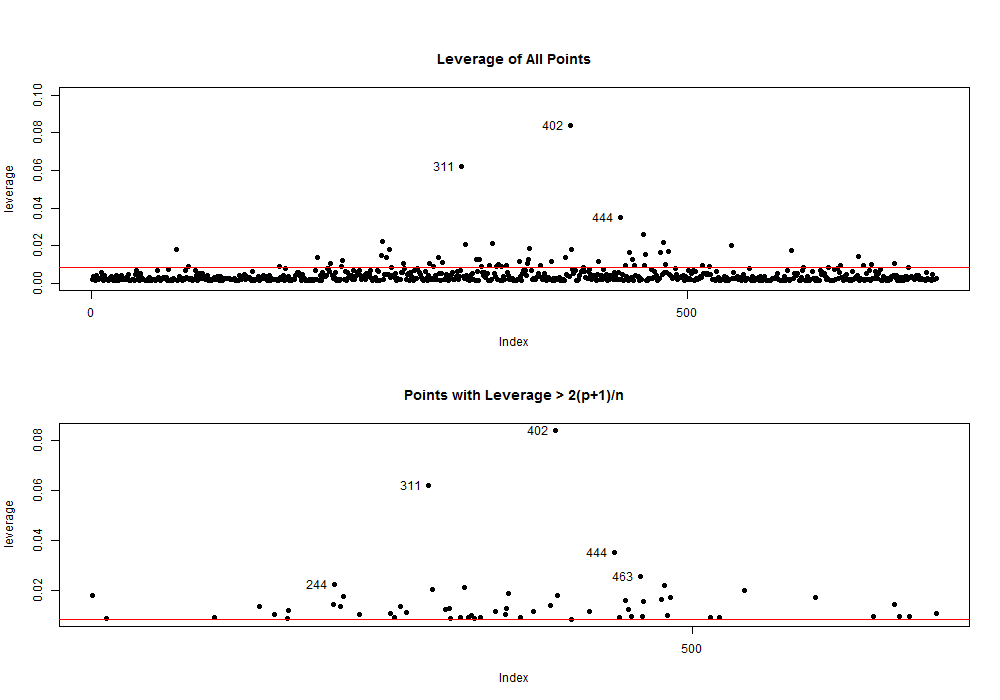
\includegraphics[width=1.3\textwidth]{charts/hw5_m1_g_leverage}
    \end{center}
    \caption{%
     Plot of the Hat Values(Leverage)  Vs Index 
     }%
   \label{fig:hw5_m1_g_leverage}
\end{figure}
}

$\\$
\FloatBarrier
\subsubsection{Diagnostics - Influence}
{
Cook's distance measures the influence of a observation point on the fitted values. Figure $\eqref{fig:hw5_m1_g_cooks}$, the scatter plot of the Square root of the cooks distance and the half normal plot show observation 402 to be having a largest influence. From the Leverage plot and the Studentized Residual plot we notice that this observation is also an residual outlier and a high leverage point. The following is the data for observation 402.
\begin{verbatim}
    Toyota    Ford     GM leverage
402 -0.113 -0.0875 -0.106    0.493
\end{verbatim}
The data shows large negative returns that seem to have affected all 3 stocks for this day. This seems to be a valid data point, showing tail dependence and that needs to be factored into the model.
\begin{figure}[htbp!]
     \begin{center}
      \hspace*{-1.4in}
           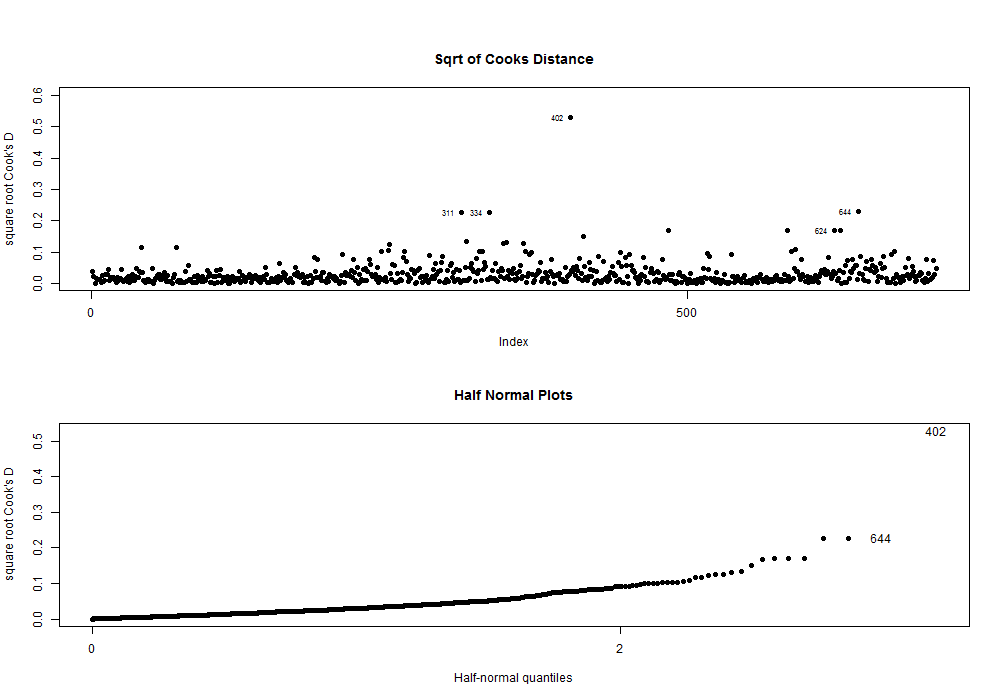
\includegraphics[width=1.4\textwidth]{charts/hw5_m1_g_cooks}
    \end{center}
    \caption{%
     Square Root Cooks Distance (Influence) - Scatter Plot Vs Index and Half Normal Plots
     }%
   \label{fig:hw5_m1_g_cooks}
\end{figure}
}

$\\$
\FloatBarrier
\subsubsection{Diagnostics - Studentized Residuals}
\label{rstudent_residuals_cooks_1}
{
Raw residuals do not have constant variance since they depend on the leverage and residual outlier position of that point.
To overcome this we use Standardized Residuals also called externally Studentized Residuals. Figure $\eqref{fig:hw5_m1_g_rstudent_residuals}$ plots the Studentized Residuals for each point Versus the Leverage and Cooks Distance for that point. High Leverage points have lower residuals and the variation in RStudent increases as the influence of the points increase.
\begin{figure}[htbp!]
     \begin{center}
     \hspace*{-1.0in}
             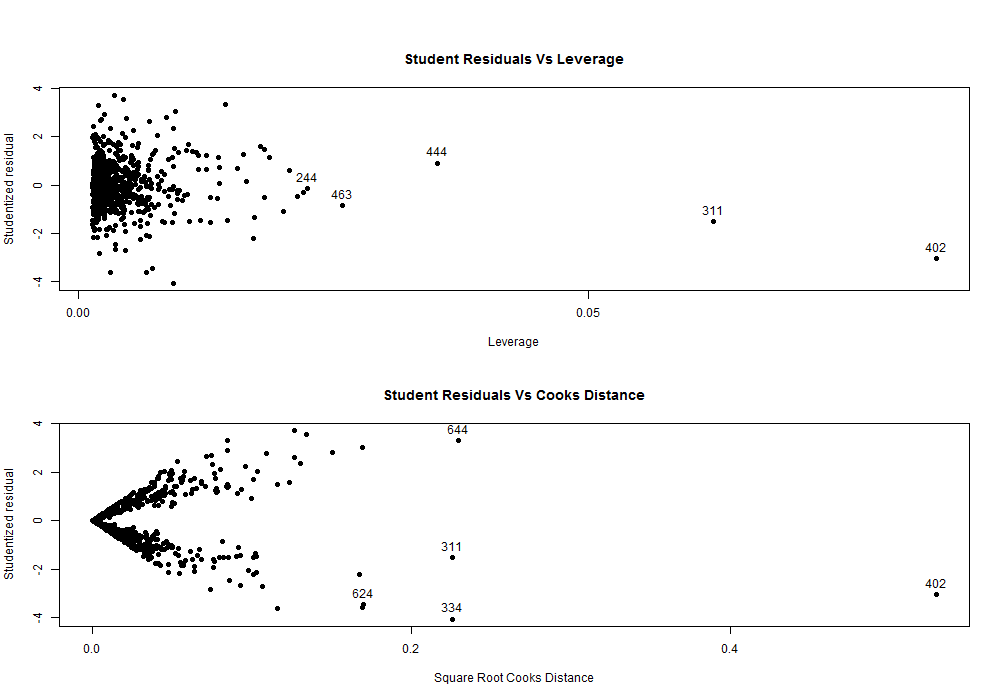
\includegraphics[width=1.3\textwidth]{charts/hw5_m1_g_rstudent_residuals}
    \end{center}
    \caption{%
     Studentized Residuals Versus Leverage and Cooks Distance
     }%
   \label{fig:hw5_m1_g_rstudent_residuals}
\end{figure}
}

\FloatBarrier
\subsubsection{Verify Model Assumptions}
\label{assumptions_lm_1}

{
Figure $\eqref{fig:Model Assumptions_1}$ plots the metrics that enable checking of the model assumptions of normality, linearity and constant variance. The density plot and the Normal QQ plot of the studentized residuals shows a thick tailed symmetric distribution. The plot of the Studentized Residuals versus Ford shows linearity, but the plot of the Studentized Residuals versus Toyota shows slight nonlinearity at the extremes. This would indicate tail dependence as discussed earlier at extreme values of returns. The plot of the Studentized Residuals versus Fitted Values is fairly linear and horizontal showing constant variance.
\begin{figure}[htbp!]
     \begin{center}
     \hspace*{-1.0in}
             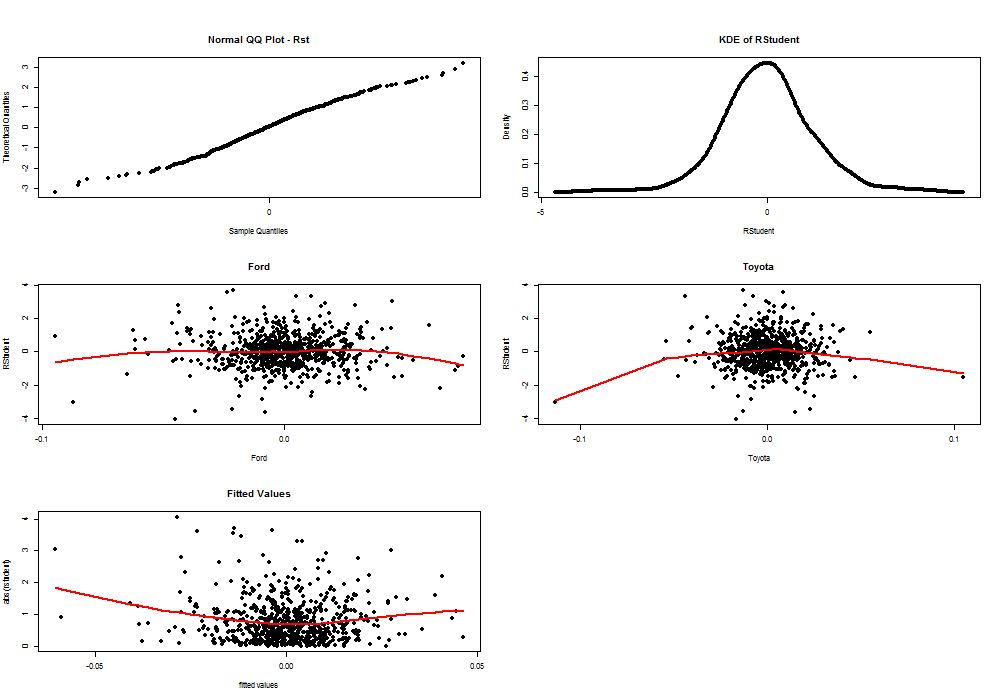
\includegraphics[width=1.4\textwidth]{charts/hw5_m1_g_heteroskedacity}
    \end{center}
    \caption{%
     Plots to check assumptions of Normality, Linearity and Constant Variance - Plot of Studentized Residuals Vs Predictors, Fitted Values
     }%
   \label{fig:Model Assumptions_1}
\end{figure}
}

$\\$
\FloatBarrier
\subsubsection{Model Summary}
\label{model_summary_1}
$\\$
The following is the summary of the simple linear regression model with 2-Predictors variables Ford and Toyota. The $\mathbf{R}^2 \approxeq 0.38$ for this model.
\begin{verbatim}

Summary for the linear regression model : GM ~ Ford + Toyota :

Call:
lm(formula = GM ~ Ford + Toyota, data = data)

Residuals:
     Min       1Q   Median       3Q      Max 
-0.06285 -0.00965 -0.00040  0.00898  0.05752 

Coefficients:
            Estimate Std. Error t value Pr(>|t|)    
(Intercept) 7.05e-05   5.91e-04    0.12     0.91    
Ford        6.14e-01   3.13e-02   19.62   <2e-16 ***
Toyota      6.13e-02   3.78e-02    1.62     0.11    
---
Signif. codes:  0 ‘***’ 0.001 ‘**’ 0.01 ‘*’ 0.05 ‘.’ 0.1 ‘ ’ 1

Residual standard error: 0.0157 on 706 degrees of freedom
Multiple R-squared:  0.377,	Adjusted R-squared:  0.376 
F-statistic:  214 on 2 and 706 DF,  p-value: <2e-16
\end{verbatim}



$\\\\$
\FloatBarrier
\subsection{Considering a Linear Model with Polynomial Terms}
\label{analysis_lm_poly}
We have seen that the correlation between Toyota and GM is very low at $0.20$. The Studentized Residual Plot versus the predictor variable Toyota in section $\eqref{assumptions_lm_1}$ shows a slight deviation from linearity at the extremes. One way to overcome this non linearity in the Studentized Residuals with predictor variable Toyota is to see if we could fit a better linear model using degree 2 polynomial terms in Toyota. The polynomial terms used will be generated by the $poly()$ function in R and will be orthonormal, as in QR distribution.
$\\\\$
The following is the correlation matrix with degree 2 polynomial terms in Toyota. It can be seen that the correlation between the 2nd degree term in Toyota and Ford is $-0.075$, which is far less than the correlation of $0.24$ between the degree 1 term in Toyota and Ford. 
\begin{verbatim}
> cor(cbind(poly(Toyota,2),Ford,GM))
            1        2   Ford    GM
1     1.0e+00 -1.9e-17  0.242  0.20
2    -1.9e-17  1.0e+00 -0.075 -0.13
Ford  2.4e-01 -7.5e-02  1.000  0.61
GM    2.0e-01 -1.3e-01  0.613  1.00
\end{verbatim}


$\\$
\FloatBarrier
\subsubsection{Model Selection - Predictor Subset}
The results of both the $leaps()$ and $regsubsets()$ functions in R which choose the best k-subset of predictors for each k are shown below. Results show that both functions choose the 2nd degree polynomial term in Toyota over the first degree term in Toyota for the 2-subset of predictor model.

\begin{verbatim}
Leaps - Best Model for each K Predictor by Cp:
  Ford Toyota1 Toyota2     
1    1       0       0 11.2
2    1       0       1  4.8
3    1       1       1  4.0


Regression Subsets - Choosing the Best set of Predictors by BIC/Cp:
Subset selection object
Call: regsubsets.formula(data$GM ~ ., data = as.data.frame(cbind(data$Ford, 
    poly(data$Toyota, 2))), nbest = 1)
3 Variables  (and intercept)
    Forced in Forced out
V1      FALSE      FALSE
`1`     FALSE      FALSE
`2`     FALSE      FALSE
1 subsets of each size up to 3
Selection Algorithm: exhaustive
         V1  `1` `2`
1  ( 1 ) "*" " " " "
2  ( 1 ) "*" " " "*"
3  ( 1 ) "*" "*" "*"
\end{verbatim}


$\\\\$
\FloatBarrier
{
We choose the best among these two 1,2 and 3-Predictor models by comparing the $\mathbf{R}^2$ results and along with AIC, BIC and $\mathbb{C}_p$ model quality measures. For  $\mathbf{R}^2$ a higher value is better, for the AIC, BIC and $\mathbb{C}_p$ a lower value indicates a better model.Figure $\eqref{fig:hw5_m2_g_model_selection}$ plots these values.
\begin{figure}[htbp!]
     \begin{center}
             \hspace*{-1.3in}
            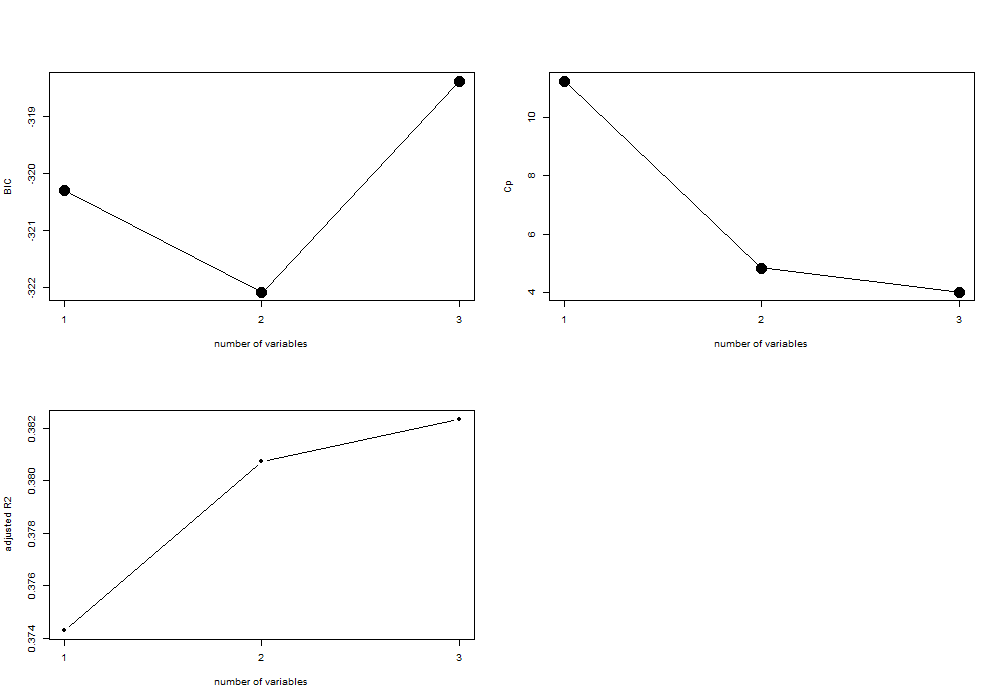
\includegraphics[width=1.4\textwidth]{charts/hw5_m2_g_complexity}
    \end{center}
    \caption{%
    Poly Term Linear Model - Plot of No of Predictor Variables Vs BIC, $\mathbf{C}_p$ , $\mathbf{R}^2$ 
     }%
   \label{fig:hw5_m2_g_model_selection}
\end{figure}
}

\FloatBarrier
\subsubsection{Model Selection - AIC }
\label{stepaic_2}
The most parsimonious model is the model with the lowest AIC value. The $stepAIC()$ R call systematically removes one predictor variable at a time till the AIC stops reducing. The following results of the $stepAIC()$ call show that the 3 predictor variable model has the lowest AIC of -5892. This is slightly lower than the AIC of -5885.44, for the earlier linear regression model without polynomial terms in Toyota in $\eqref{stepaic_1}$.

\begin{verbatim}
Step AIC  GM ~ Ford + poly(Toyota, 2) :
Start:  AIC=-5892
GM ~ Ford + poly(Toyota, 2)

                  Df Sum of Sq   RSS   AIC
<none>                         0.172 -5892
- poly(Toyota, 2)  2    0.0027 0.175 -5885
- Ford             1    0.0924 0.265 -5590
\end{verbatim}

$\\\\$
\FloatBarrier
\subsubsection{ANOVA}
The following are the ANOVA results of the linear regression model with degree 2 polynomial terms in Toyota. The F-Value for the Poly terms in Toyota is much smaller at $\approxeq .4\%$. Thus we can confidently reject the null hypothesis and take the model with the Poly term in Toyota as significant. 
\begin{verbatim}
ANOVA for the linear regression model : GM ~ Ford + poly(Toyota, 2) :
Analysis of Variance Table

Response: GM
                 Df Sum Sq Mean Sq F value Pr(>F)    
Ford              1 0.1052  0.1052  430.05 <2e-16 ***
poly(Toyota, 2)   2 0.0027  0.0014    5.62 0.0038 ** 
Residuals       705 0.1724  0.0002                   
---
Signif. codes:  0 ‘***’ 0.001 ‘**’ 0.01 ‘*’ 0.05 ‘.’ 0.1 ‘ ’ 1
\end{verbatim}


$\\\\$
The following are ANOVA the results comparing the 2 models. Again the F-Value for the Poly terms model is  much smaller at $\approxeq .35\%$. Thus we can confidently reject the null hypothesis and take the linear model with the Polynomial term in Toyota as significant.
\begin{verbatim}
Comparing Models by ANOVA:
Analysis of Variance Table
Model 1: GM ~ Ford + Toyota
Model 2: GM ~ Ford + poly(Toyota, 2)
  Res.Df   RSS Df Sum of Sq    F Pr(>F)   
1    706 0.174                            
2    705 0.172  1    0.0021 8.58 0.0035 **
---
Signif. codes:  0 ‘***’ 0.001 ‘**’ 0.01 ‘*’ 0.05 ‘.’ 0.1 ‘ ’ 1
\end{verbatim}


$\\$
\FloatBarrier
\subsubsection{Diagnostics - Leverage}
\label{diagnostics_leverage_2}
The number of high leverage points with this model is 41, ie, there 41 high leverage points with leverage $>= \frac{2(p+1)}{n}$ where $\frac{(p+1)}{n}$ is the average leverage. This is less than the 59 high leverage points that we had with the earlier model in $\eqref{diagnostics_leverage_1}$

$\\$
\FloatBarrier
\subsubsection{Diagnostics - Studentized Residuals}
{
 The plot of the Studentized Residuals for each point Versus the Leverage and Cooks Distance for that point in figure $\eqref{fig:hw5_m2_g_rstudent_residuals}$ shows much less spread than a similar plot for the earlier model in $\eqref{rstudent_residuals_cooks_1}$ 
\begin{figure}[htbp!]
     \begin{center}
     \hspace*{-1.1in}
             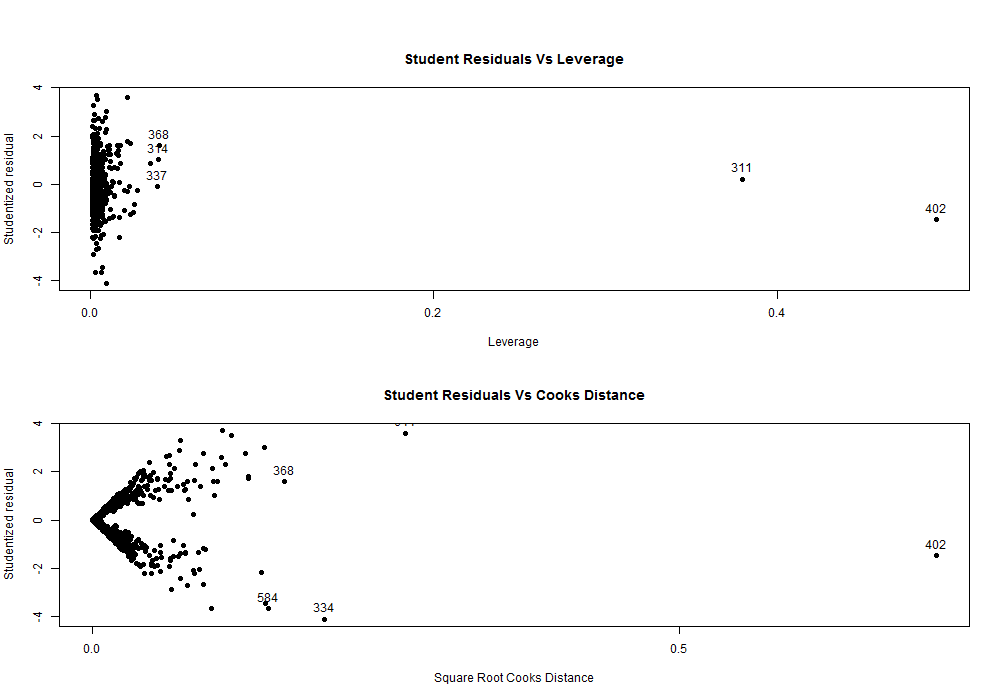
\includegraphics[width=1.35\textwidth]{charts/hw5_m2_g_rstudent_residuals}
    \end{center}
    \caption{%
     Poly Term Linear Model - Studentized Residuals Versus Leverage and Cooks Distance
     }%
   \label{fig:hw5_m2_g_rstudent_residuals}
\end{figure}
}

$\\\\$
\FloatBarrier
\subsubsection{Model Assumptions}
\label{assumptions_lm_2}
{
Figure $\eqref{fig:Model Assumptions2}$ plots the metrics that enable checking of the model assumptions of normality, linearity and constant variance. The plot of the Studentized Residuals versus Toyota as well as the Studentized Residuals versus Fitted Values shows better linearity with this model than the similar plot for the earlier model in section $\eqref{assumptions_lm_1}$. This indicates better linearity and better constant variance with this model.
\begin{figure}[htbp!]
     \begin{center}
     \hspace*{-1.2in}
             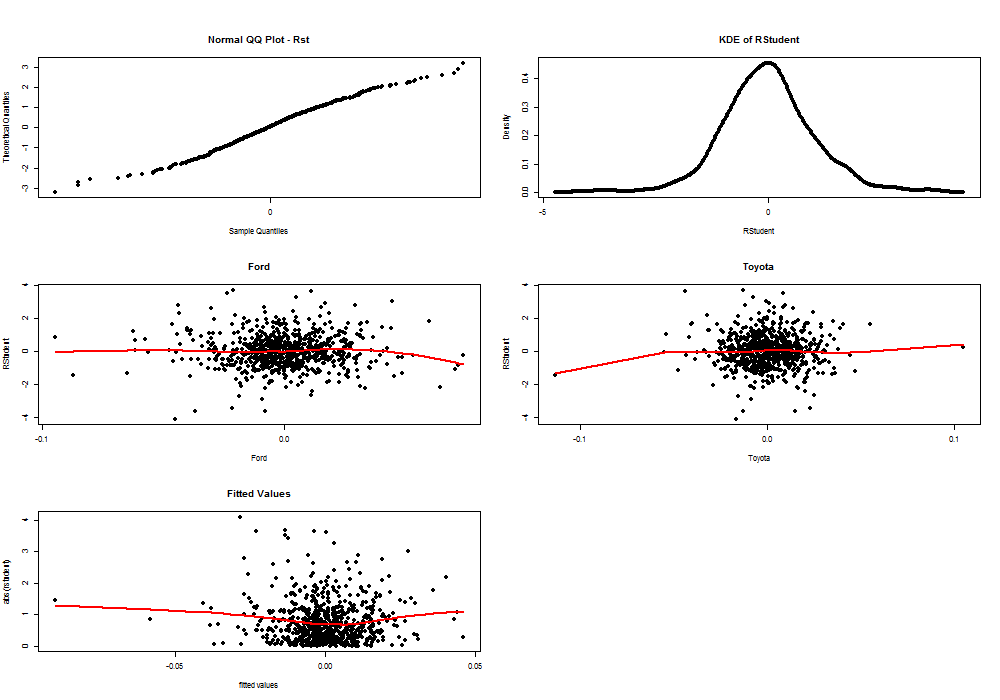
\includegraphics[width=1.35\textwidth]{charts/hw5_m2_g_heteroskedacity}
    \end{center}
    \caption{%
     Poly Term Linear Model - Plots to check assumptions of Normality, Linearity and Constant Variance - Plot of Studentized Residuals Vs Predictors, Fitted Values
     }%
   \label{fig:Model Assumptions2}
\end{figure}
}

$\\$
\FloatBarrier
\subsubsection{Compare Model Summary}
\label{model_summary_2}
The following is the summary of the linear regression model degree 2 Polynomial terms in Toyota. As can be seen the P-value is $\approxeq 0.35\%$ for the 2nd degree polynomial term in Toyota. Thus we can confidently reject the null hypothesis and accept the 2nd degree polynomial term as significant to the model. The $\mathbf{R}^2 \approxeq 0.39$ for this model. This is a slight improvement compared to the  $\mathbf{R}^2 \approxeq 0.38$ value for the earlier model in $\eqref{model_summary_1}$.
\begin{verbatim}
Summary for the linear regression model : GM ~ Ford + poly(Toyota, 2) :

Call:
lm(formula = GM ~ Ford + poly(Toyota, 2))

Residuals:
     Min       1Q   Median       3Q      Max 
-0.06315 -0.00974 -0.00046  0.00866  0.05712 

Coefficients:
                  Estimate Std. Error t value Pr(>|t|)    
(Intercept)       0.000124   0.000587    0.21   0.8324    
Ford              0.607437   0.031248   19.44   <2e-16 ***
poly(Toyota, 2)1  0.027149   0.016123    1.68   0.0927 .  
poly(Toyota, 2)2 -0.045947   0.015686   -2.93   0.0035 ** 
---
Signif. codes:  0 ‘***’ 0.001 ‘**’ 0.01 ‘*’ 0.05 ‘.’ 0.1 ‘ ’ 1

Residual standard error: 0.016 on 705 degrees of freedom
Multiple R-squared:  0.385,	Adjusted R-squared:  0.382 
F-statistic:  147 on 3 and 705 DF,  p-value: <2e-16

\end{verbatim}


$\\\\$
\FloatBarrier
\subsection{10 Fold Cross Validation - Evaluate Models}
\label{10_fold_cv}
{
While the analysis so far indicates that the linear regression model with polynomial terms in Toyota is  better than the simple linear regression model with only first degree terms in Ford and Toyota, the robust way to validate these models is by performing a 10 fold cross validation on them.  In each fold the model is trained on the training set and the results are recorded on the hold out validation set. The Mean of the residual sum of squares across all the validation sets is computed as MSE. This statistic MSE is used to compared the performance of the models. The following are the MSE results for the two models using 10 fold cross validation. The Figure $\eqref{fig:hw5_cv}$ plots the MSE for each of the models at each fold of cross validation.

\begin{verbatim}
Results of 10 Fold Cross Valiation: MSE on the Validation Set for Each Model:
Model : GM ~ Ford + Toyota
MSE= 0.000251
Model : GM ~ Ford + poly(Toyota, 2)
MSE= 0.000248
\end{verbatim}
\begin{figure}[htbp!]
     \begin{center}
     \hspace*{-1.05in}
            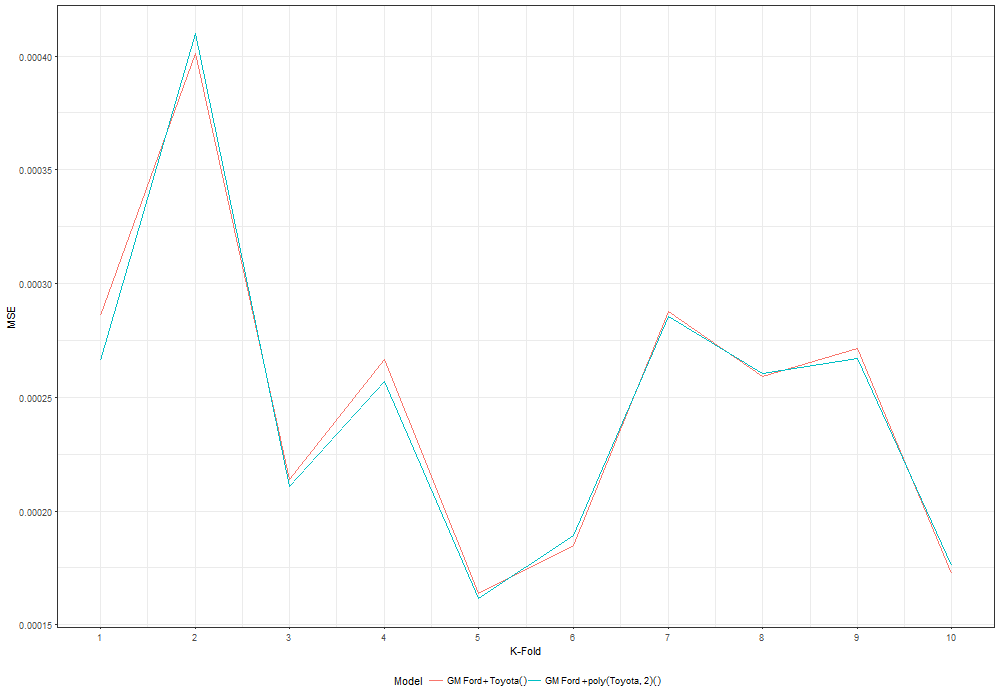
\includegraphics[width=1.38\textwidth]{charts/hw5_cv_plot}
    \end{center}
    \caption{%
     10 Fold Cross Validation Results - Comparison of Poly(Toyota,2) and Non Poly Term Models - Validation Set MSE for each Fold
     }%
   \label{fig:hw5_cv}
\end{figure}
}




$\\\\$
\FloatBarrier
\section{Conclusion}
\label{conclusion}
\begin{itemize}
\item
As seen from the results of the 10 fold cross validation in section $\eqref{10_fold_cv}$ the linear regression model with 2nd degree Poly terms in Toyota has a slightly better performance. It has a lower MSE of 0.000248 compared to a MSE of 0.000251 for the linear regression model without any Poly terms. The plot $\eqref{fig:hw5_cv}$ of the MSE at each fold in the cross validation also corroborates that the linear regression model with 2nd degree Poly terms in Toyota has a lower MSE for most of the folds.
\item
The Poly term in the linear regression model increases the model complexity by adding an additional parameter. So the models need to be compared using a measure of relative model quality like AIC. From the AIC values in section $\eqref{stepaic_2}$ we see that the linear regression model with degree 2 polynomial terms in Toyota as a AIC of -5892  compared to AIC of -5885.44, for the linear regression model without polynomial terms in Toyota in $\eqref{stepaic_1}$. Thus the Linear Regression Model with degree 2 polynomial terms in Toyota has a slightly better AIC.
\item
In section $\eqref{model_summary_2}$ we see that the Linear Regression Model with degree 2 polynomial terms in Toyota has $\mathbf{R}^2 \approxeq 0.39$ which is a slight improvement compared to the  $\mathbf{R}^2 \approxeq 0.38$ value for the  linear regression model without polynomial terms.
\item
We see in section $\eqref{diagnostics_leverage_2}$ that the Linear Regression Model with degree 2 polynomial terms in Toyota has fewer high leverage points than the linear regression model without polynomial terms.
\item
In section $\eqref{assumptions_lm_2}$ we see that that the Linear Regression Model with degree 2 polynomial terms in Toyota  has better linearity and constant variance characteristics than the linear regression model without polynomial terms.
\item
Thus we conclude that the following Linear Regression Model with degree 2 polynomial terms in Toyota is the better model for the sample data set provided for predicting the log returns for GM , from the log returns of Ford and Toyota as the predictors.
\begin{verbatim}
GM ~ Ford + poly(Toyota, 2):
 llfit$coefficients
     (Intercept)             Ford poly(Toyota, 2)1 poly(Toyota, 2)2 
         0.00012          0.60744          0.02715         -0.04595 
\end{verbatim}
\end{itemize}

$\\\\$
\FloatBarrier
\begin{appendices}
\label{appendix}
The source code for data analysis, for generating the 2 linear regression models and for evaluating the models is in file $hw5\_1.R$. This source code is also attached below.
\begin{lstlisting}

#########################################################################################
###########  ISYE6783         ######
###########  DL  Ajay DSouza   #####
###########   HW 5            ######
#########################################################################################

library(leaps)
library(faraway)
library(MASS)
library(car)
library(reshape2)
library(ggplot2)

#--------------------------------------------
# Setup
#
#--------------------------------------------

#cleanup
rm(list = ls())

# set rounding digits globally
options(digits = 6)

set.seed(100)

#setwd(
#  "C:/wk/odrive/Amazon Cloud Drive/ajays_stuff/georgia_tech_ms/isye_math6783_financial_data_analysis/hw5"
#)

sink("hw5_script_output.txt", append = FALSE, split = TRUE)
sink()


sink("hw5_script_output.txt", append = TRUE, split = TRUE)
cat('\nHW5\n')
sink()

# Read the ascii data file
data <-
  read.csv(file = "w_logret_3automanu.csv", header = FALSE, sep =
             ",")


# N data size
n <- nrow(data)

# set column names
colnames(data) <- c('Toyota', 'Ford', 'GM')

#attach data
detach(data)
attach(data)

# ------------------------------------------
# Data Analysis
# ------------------------------------------
# 1 scatter plot
par(mfrow = c(1, 1))
scatterplotMatrix( ~ GM + Ford + Toyota, main = "")
dev.copy(png,
         filename = "hw5_g_pairs.png",
         width = 1000,
         height = 700)
dev.off()

# correlation
sink("hw5_script_output.txt", append = TRUE, split = TRUE)
cat(paste("\n\n\nCorrelation:\n"))
print(cor(data))
sink()


sink("hw5_script_output.txt", append = TRUE, split = TRUE)
cat(paste("\n\n\nCorrelation With poly(Toyota,2):\n"))
print( cor(cbind(poly(Toyota,2),Ford,GM)))
sink()

# 2 Histogram, KDE
par(mfrow = c(3, 1), oma = c(0, 0, 2, 0))
den <- density(data$Toyota)
plot(den$x, den$y, xlab = "Toyota", ylab = "Density")

den <- density(data$Ford)
plot(den$x, den$y, xlab = "Ford", ylab = "Density")

den <- density(data$GM)
plot(den$x, den$y, xlab = "GM", ylab = "Density")

#title("Density(KDE) Plot - Daily Log Returns", outer = TRUE)

dev.copy(png,
         filename = "hw5_g_kde.png",
         width = 1000,
         height = 700)
dev.off()



# 3 QQplot with normal distribution
# qqplot with T distribution
tqd <- pt((seq(n) - .5) / n, df = 2.4)

par(mfrow = c(3, 2), oma = c(0, 0, 2, 0))
qqnorm(data$Toyota,
       datax = TRUE,
       ylab = "Toyota",
       main = "QQNorm")
qqplot(data$Toyota, tqd, xlab = "Toyota", main = "QQ-TDist")

qqnorm(data$Ford,
       datax = TRUE,
       ylab = "Ford",
       main = "QQNorm")
qqplot(data$Ford, tqd, xlab = "Ford", main = "QQ-TDist")

qqnorm(data$GM,
       datax = TRUE,
       ylab = "GM",
       main = "QQNorm")
qqplot(data$GM, tqd, xlab = "GM", main = "QQ-TDist")

#title("QQPlot\n Normal , T-Distribution \n Daily Log Returns", outer = TRUE)

dev.copy(png,
         filename = "hw5_g_qq.png",
         width = 1000,
         height = 700)
dev.off()


#------------------------------------------------------
# Linear Regression - Model 1 - Analysis
# lm (GM~Ford+Toyota)
#
#------------------------------------------------------

for (mdel in c(1, 2)) {
  #annova
  if (mdel == 1) {
    llfit <- lm(data = data, GM ~ Ford + Toyota)
  }
  else if (mdel == 2) {
    lofit <- llfit
    llfit <- lm(GM ~ Ford + poly(Toyota, 2))
  }
  
  anlfit <- anova(llfit)
  
  sink("hw5_script_output.txt",
       append = TRUE,
       split = TRUE)
  cat(paste(
    "\n\n\nANOVA for the linear regression model :",
    llfit$call[2],
    ":\n"
  ))
  print(anlfit)
  sink()
  
  #summary
  smlfit <- summary(llfit)
  sink("hw5_script_output.txt",
       append = TRUE,
       split = TRUE)
  cat(paste(
    "\n\n\nSummary for the linear regression model :",
    llfit$call[2],
    ":\n"
  ))
  print(smlfit)
  sink()
  

  
  # Anova comparison of two models and F
  if (mdel == 1) {
    llfit2 <- lm(data = data, GM ~ Ford)
    acomp <- anova(llfit2, llfit)
    
  } else if (mdel == 2) {
    acomp <- anova(lofit,llfit)
  }
  
  sink("hw5_script_output.txt",
       append = TRUE,
       split = TRUE)
  cat(paste("\n\n\nComparing Models by ANOVA:\n"))
  print(acomp)
  sink()
  
  

  # Model Selection
  if (mdel == 1) {
    subsets = regsubsets(data$GM ~ .,
                         data = as.data.frame(cbind(data$Ford, data$Toyota)), nbest =
                           1)
  } else if (mdel == 2) {
    subsets = regsubsets(data$GM ~ .,
                         data = as.data.frame(cbind(data$Ford, poly(data$Toyota, 2))), nbest =
                           1)
  }
  
  b = summary(subsets)
  
  sink("hw5_script_output.txt",
       append = TRUE,
       split = TRUE)
  cat(
    paste(
      "\n\n\nRegression Subsets - Choosing the Best set of Predictors by BIC/Cp:\n"
    )
  )
  print(b)
  sink()
  
  
  
  nms <- length(coef(llfit)) - 1
  
  par(
    mfrow = c(2, 2),
    oma = c(0, 0, 2, 0),
    lab = c(2, 5, 3),
    pch = 19
  )
  plot(
    1:nms,
    b$bic,
    type = "b",
    xlab = "number of variables",
    ylab = "BIC",
    cex = 2.5
  )
  plot(
    1:nms,
    b$cp,
    type = "b",
    xlab = "number of variables",
    ylab = "Cp",
    cex = 2.5
  )
  plot(1:nms,
       b$adjr2,
       type = "b",
       xlab = "number of variables",
       ylab = "adjusted R2")
  #title(paste("Model Selection - \nDaily Log Returns ", llfit$call[2]),
  #      outer = TRUE)
  dev.copy(
    png,
    filename = paste("hw5_m", mdel, "_g_complexity.png", sep = ""),
    width = 1000,
    height = 700
  )
  dev.off()
  
  
  #vif for collenarity
  vf <- vif(lm(llfit))
  sink("hw5_script_output.txt",
       append = TRUE,
       split = TRUE)
  cat(paste("\n\n\nVariance Inflation Factor:\n"))
  print(vf)
  sink()
  
  
 
  #StepAIC
  
  sink("hw5_script_output.txt",
       append = TRUE,
       split = TRUE)
  cat(paste("\n\n\nStep AIC ", llfit$call[2], ":\n"))
  step_lm = stepAIC(llfit)
  cat("\n\n")
  smlm <- summary(lm(step_lm))
  print(smlm)
  sink()
  

  #leaps
  if (mdel == 1) {
    x1 = as.matrix(cbind(Ford, Toyota))
    names_x1 = c("Ford", "Toyota")
  } else if (mdel == 2) {
    x1 = as.matrix(cbind(Ford, poly(Toyota, 2)))
    names_x1 = c("Ford", "Toyota1", "Toyota2")
  }
  
  leaps.fit = leaps(
    y = GM,
    x = x1,
    names = names_x1,
    nbest = 1
  )
  options(digits = 2)
  
  sink("hw5_script_output.txt",
       append = TRUE,
       split = TRUE)
  cat(paste("\n\n\nLeaps - Best Model for each K Predictor by Cp:\n"))
  print(cbind(leaps.fit$which, leaps.fit$Cp))
  sink()
  

  
  # Partial Residual Plots
  par(
    mfrow = c(2, 2),
    oma = c(0, 0, 2, 0),
    lab = c(2, 5, 3),
    pch = 19
  )
  lfit_ford = lm(GM ~ Ford)
  lfit_toyota = lm(GM ~ Toyota)
  crPlot(
    llfit,
    var = "Ford",
    main = "Partial - Ford",
    smooth = F,
    lty = 1,
    lwd = 2,
    col = "black"
  )
  
  if (mdel == 1) {
    crTVar <- 'Toyota'
  } else if (mdel == 2) {
    crTVar <- 'poly(Toyota, 2)'
  }
  crPlot(
    llfit,
    var = crTVar,
    main = paste("Partial-", crTVar),
    smooth = F,
    lty = 1,
    lwd = 2,
    col = "black"
  )
  plot(Ford, GM, main = "Ford Vs GM")
  regLine(lfit_ford,
          col = "red",
          lwd = 2,
          lty = "dashed")
  plot(Toyota, GM, main = "Toyota Vs GM")
  regLine(lfit_toyota,
          col = "red",
          lwd = 2,
          lty = "dashed")
  #title(paste("Partial Residual Plots- \nDaily Log Returns ", llfit$call[2]),
  #      outer = TRUE)
  dev.copy(
    png,
    filename = paste("hw5_m", mdel, "_g_partial_residual.png", sep =
                       ""),
    width = 1000,
    height = 700
  )
  dev.off()
  
  # High Leverage Points
  hvals <- hatvalues(llfit)
  # High leverage points > 2(p+1)/n more than 2wice the average ( 59 of them)
  hLevAv <- (length(coef(llfit)) - 1 + 1) / length(llfit$residuals)
  hValHAvg <- sum(hvals > 2 * hLevAv)
  sIdx <- sort(hvals, decreasing = TRUE, index.return = TRUE)
  
  # Top 5 high leverage points
  tp <- 10
  sink("hw5_script_output.txt",
       append = TRUE,
       split = TRUE)
  cat(paste("\n\n\nTop ", tp, " Data Points with the Highest Leverage:\n"))
  print(cbind(data[head(unique(sIdx$ix), tp), ], leverage = head(unique(sIdx$x), tp)))
  
  cat(paste(
    "\n\n\nThe Correlation between the ",
    hValHAvg,
    " High Leverage Data Points:\n"
  ))
  print(cor(cbind(data[head(unique(sIdx$ix), hValHAvg), ])))
  sink()
  
  
  #plot
  par(
    mfrow = c(2, 1),
    oma = c(0, 0, 2, 0),
    lab = c(2, 5, 3),
    lwd = 1,
    pch = 19
  )
  
  plot(
    hvals,
    ylab = "leverage",
    main = "Leverage of All Points",
    ylim = c(0, .1),
    xlab = "Index"
  )
  abline(h = 2 * (length(coef(llfit)) - 1 + 1) / length(llfit$residuals),
         col = 'red')
  
  gpts <-
    as.data.frame(cbind(head(unique(sIdx$ix), 3), hvals[head(unique(sIdx$ix), 3)]))
  colnames(gpts) <- c('Index', 'Leverage')
  text(gpts$Index, gpts$Leverage, gpts$Index, pos = 2)
  
  plot(
    which(hvals > 2 * (length(coef(
      llfit
    )) - 1 + 1) / length(llfit$residuals)),
    hvals[hvals > 2 * (length(coef(llfit)) - 1 + 1) / length(llfit$residuals)],
    main = paste("Points with Leverage > 2(p+1)/n"),
    ylab = "leverage",
    xlab = "Index"
  )
  abline(h = 2 * hLevAv, col = 'red')
  
  # Label the top 5 Leverage values
  gpts <-
    as.data.frame(cbind(head(unique(sIdx$ix), 5), hvals[head(unique(sIdx$ix), 5)]))
  colnames(gpts) <- c('Index', 'Leverage')
  text(gpts$Index, gpts$Leverage, gpts$Index, pos = 2)
  
  #title(paste("Leverage (Hat Values)- \nDaily Log Returns", llfit$call[2]),
  #      outer = TRUE)
  dev.copy(
    png,
    filename = paste("hw5_m", mdel, "_g_leverage.png", sep = ""),
    width = 1000,
    height = 700
  )
  dev.off()
  

  # RStudent Residuals
  
  # Studentized Residuals
  rst <- rstudent(llfit)
  
  # Label the top 5 Leverage values
  rlpts <-
    as.data.frame(cbind(head(unique(sIdx$ix), 5), hvals[head(unique(sIdx$ix), 5)], rst[head(unique(sIdx$ix), 5)]))
  colnames(rlpts) <- c('Index', 'Leverage', 'rst')
  
  # Cook's Distance
  sqcdis <- sqrt(cooks.distance(llfit))
  
  # Cook's Distance Plots
  sqcdis <- sqrt(cooks.distance(llfit))
  
  # Label the top 5 Leverage values
  cIdx <- sort(sqcdis, decreasing = TRUE, index.return = TRUE)
  
  clpts <-
    as.data.frame(cbind(head(unique(cIdx$ix), 5), hvals[head(unique(cIdx$ix), 5)], rst[head(unique(cIdx$ix), 5)], sqcdis[head(unique(cIdx$ix), 5)]))
  colnames(clpts) <- c('Index', 'Leverage', 'rst', 'Cooks')
  
    
  par(
    mfrow = c(2, 1),
    oma = c(0, 0, 2, 0),
    lab = c(2, 5, 3),
    lwd = 1,
    pch = 19
  )
  
  #plot(rst, ylab = "Studentized residual", main = "Externally Studentized Residuals")
  #plot(residuals(llfit), ylab = "residual", main = "Raw Residuals")
  plot(hvals,
       rst,
       ylab = "Studentized residual",
       xlab = "Leverage",
       main = "Student Residuals Vs Leverage")

  text(rlpts$Leverage, rlpts$rst, rlpts$Index, pos = 3)
  
  plot(sqcdis,
       rst,
       ylab = "Studentized residual",
       xlab = "Square Root Cooks Distance",
       main = "Student Residuals Vs Cooks Distance")
  
  text(clpts$Cooks, clpts$rst, clpts$Index, pos = 3)
  
  
 # title(paste("Studentized Residuals- \nDaily Log Returns ", llfit$call[2]),
 #        outer = TRUE)
  
  dev.copy(
    png,
    filename = paste("hw5_m", mdel, "_g_rstudent_residuals.png", sep =
                       ""),
    width = 1000,
    height = 700
  )
  dev.off()
  
  

  
  
  
  
  # Cooks Distance Plots  
  par(
    mfrow = c(2, 1),
    oma = c(0, 0, 2, 0),
    cex.axis = 1,
    cex.lab = 1,
    lwd = 1,
    pch = 19
  )
  
  plot(
    sqcdis,
    ylab = ("square root Cook's D"),
    cex = 1,
    main = "Sqrt of Cooks Distance",
    ylim = c(0, .6)
  )
  text(clpts$Index,
       clpts$Cooks,
       clpts$Index,
       pos = 2,
       cex = 0.7)
  
  halfnorm(
    sqcdis,
    ylab = ("square root Cook's D"),
    cex = 1,
    main = "Half Normal Plots"
  )
  
  #title(paste(
  #  "Cook's Distance- Daily Log Returns GM~Ford,Toyota",
  #  llfit$call[2]
  #),
  #outer = TRUE)
  dev.copy(
    png,
    filename = paste("hw5_m", mdel, "_g_cooks.png", sep = ""),
    width = 1000,
    height = 700
  )
  dev.off()
  
  
  
  # Check for non constant variance or heteroskedacity
  #
  # Plot of absolute Residuals versus predictors and response
  #
  
  par(
    mfrow = c(3, 2),
    oma = c(0, 0, 2, 0),
    lab = c(2, 5, 3),
    lwd = 1,
    pch = 19
  )
  arst <- abs(rst)
  
  qqnorm(rst, datax = T, main = "Normal QQ Plot - Rst")
  
  den <- density(rst)
  plot(den$x,
       den$y,
       xlab = "RStudent",
       ylab = "Density",
       main = "KDE of RStudent")
  
  plot(Ford,
       rst,
       main = "Ford",
       ylab = "RStudent",
       xlab = "Ford")
  fit2 = loess(rst ~ Ford)
  ordx2 = order(Ford)
  lines(Ford[ordx2], fit2$fitted[ordx2], col = "red", lwd = 2)
  
  plot(Toyota,
       rst,
       main = "Toyota",
       ylab = "RStudent",
       xlab = "Toyota")
  fit3 = loess(rst ~ Toyota)
  ordx2 = order(Toyota)
  lines(Toyota[ordx2], fit3$fitted[ordx2], col = "red", lwd = 2)
  
  plot(llfit$fitted,
       arst,
       xlab = "fitted values",
       ylab = "abs(rstudent)",
       main = "Fitted Values")
  fit4 = loess(arst ~ llfit$fitted)
  ord = order(llfit$fitted)
  lines(llfit$fitted[ord], fit4$fitted[ord], col = "red", lwd = 2)
  

  
 # title(
 #    paste(
 #    "Check for Variance \nResiduals Vs Predictors/Fitted Values \nDaily Log Returns ",
 #    llfit$call[2]
 #   ),
 #  outer = TRUE
 # )
  dev.copy(
    png,
    filename = paste("hw5_m", mdel, "_g_heteroskedacity.png", sep =
                       ""),
    width = 1000,
    height = 700
  )
  dev.off()
  

  # Plot the final fit
  par(
    mfrow = c(2, 2),
    oma = c(0, 0, 2, 0),
    lab = c(2, 5, 3),
    lwd = 1,
    pch = 19
  )
  
  plot(llfit)
  
  dev.copy(
    png,
    filename = paste("hw5_m", mdel, "_g_fit.png", sep = ""),
    width = 1000,
    height = 700
  )
  dev.off()
  
}

#--------------------------------------------
#
# Model Comparison
#
# 10 fold cross validation of the chosen models
#
#--------------------------------------------
# Split data into train and hold out test
#

# Number of folds
nFolds <- 10

#Randomly shuffle the array index
smpIdx <- sample(n)

#Create 10 equally size folds
folds <- cut(seq(1, n), breaks = nFolds, labels = FALSE)

# Store the fold results
fResults <- data.frame(
  model = integer(),
  k = integer(),
  trainN = integer(),
  testN = integer(),
  SSR = double(),
  SSE = double(),
  SST = double(),
  MSE = double(),
  MST = double(),
  R2 = double(),
  R2A = double(),
  MSET = double(),
  corFitTrain = double(),
  corTestFit = double(),
  stringsAsFactors = FALSE
)

for (mdel in c(1:2)) {
  #Perform 10 fold cross validation
  for (k in 1:10) {
    testIndices <- smpIdx[which(folds == k, arr.ind = TRUE)]
    ## pick a random train and test rows
    testData <- data[testIndices,]
    trainData <-  data[-testIndices,]
    
    # perform linear regression
    if (mdel == 1) {
      lfit <- lm(data = trainData, GM ~ Ford + Toyota)
    }
    else if (mdel == 2) {
      # perform linear regression
      lfit <- lm(data = trainData, GM ~ Ford + poly(Toyota, 2))
    }
    
    
    # residual - mean square error on the fitted data
    yTrainBar <- mean(trainData$GM)
    nTrain <- length(trainData$GM)
    
    #SSR
    SSR <- sum((predict(lfit) - yTrainBar) ^ 2)
    
    #SSE and MSE
    SSE <-  sum(lfit$residuals ^ 2)
    MSE <- SSE / df.residual(lfit)
    
    # SST and MST
    SST <- sum((trainData$GM - yTrainBar) ^ 2)
    MST <- SST / (nTrain - 1)
    
    # MSE on the training data
    nTest <- length(testData$GM)
    testPred <- predict.lm(lfit, testData[, c('Ford', 'Toyota')])
    MSET <- sum((testPred - testData$GM) ^ 2) / nTest
    
    
    # Save the results
    fResults[nrow(fResults) + 1,] <- c(
      mdel,
      k,
      nTrain,
      nTest,
      SSR,
      SSE,
      SST,
      MSE,
      MST,
      SSR / SST,
      1 - (MSE / MST),
      MSET,
      cor(lfit$fitted.values, trainData$GM) **
        2,
      cor(testPred, testData$GM) ** 2
    )
  }
}

CV_MSE_1 <-
  sum(fResults[fResults$model == 1, ]$MSET * fResults[fResults$model == 1, ]$testN) /
  n
CV_MSE_2 <-
  sum(fResults[fResults$model == 2, ]$MSET * fResults[fResults$model == 2, ]$testN) /
  n


sink("hw5_script_output.txt", append = TRUE, split = TRUE)
cat(
  paste(
    "\n\n\n\nResults of 10 Fold Cross Valiation: MSE on the Validation Set for Each Model:\n"
  )
)
cat(paste("\nModel :", lofit$call[2]))
cat(paste("\nMSE=", round(CV_MSE_1, 6)))
cat(paste("\n"))
cat(paste("\nModel :", llfit$call[2]))
cat(paste("\nMSE=", round(CV_MSE_2, 6)))
cat(paste("\n"))
sink()

fResults$model <- as.factor(fResults$model)

#melt with method name as pivot
molten <-
  melt(
    fResults[, c('k', 'model', 'MSET')],
    id.vars = c('model', 'k'),
    measure.vars = c('MSET'),
    variable_name = 'series'
  )


klabs <- c(paste(unlist(seq(1:10))))

par(
  mfrow = c(1, 1),
  oma = c(0, 0, 2, 0),
  lab = c(2, 5, 3),
  lwd = 1,
  pch = 19
)

ggplot(molten, aes(x = k, y = value, colour = model)) +
  geom_line() +
  scale_x_continuous(breaks = 1:10, labels = klabs) +
  xlab("K-Fold") +
  ylab("MSE") +
  scale_colour_discrete(
    name  = "Model",
    breaks = c("1", "2"),
    labels = c(lofit$call[2], llfit$call[2])
  ) +
  scale_shape_discrete(
    name  = "Model",
    breaks = c("1", "2"),
    labels = c(lofit$call[2], llfit$call[2])
  ) +
  ggtitle(paste("10 Fold Validation, MSE on Validation Set")) +
  theme_bw() +
  theme(plot.title = element_text(hjust = 0.5),
        legend.position = "bottom")

dev.copy(png,
         filename = "hw5_cv_plot.png",
         width = 1000,
         height = 700)
dev.off()


#----------------------------------------------
# END
#----------------------------------------------

\end{lstlisting}

\end{appendices}



$\\\\$
%\addcontentsline{toc}{section}{References}
\bibliographystyle{unsrt}
\bibliography{sample}
%\bibliographystyle{plain}
% Generate the bibliography.
\begin{thebibliography}{9}

\bibitem{ruppert_2015}
  Ruppert David, Matteson S. David,
  \emph{Statistics and Data Analysis for Financial Engineering},
  Springer-Verlag New York Edition 2,
  2015.

\end{thebibliography}

\end{document}